\documentclass{beamer}
\usepackage{amsmath, amssymb}
\usepackage{graphicx}
\usepackage{listings}
\usepackage{color}
\usepackage{subfig}
\usepackage{hyperref}
\usepackage{tcolorbox,fancyvrb,xcolor,tikz}
\tcbuselibrary{skins,breakable}

\newenvironment{VerbatimIN}
 {\VerbatimEnvironment
  \begin{tcolorbox}[
    breakable,
    colback=lightgray,
    spartan
  ]%
  \begin{Verbatim}}
 {\end{Verbatim}\end{tcolorbox}}

 \newenvironment{VerbatimOUT}
 {\VerbatimEnvironment
  \begin{tcolorbox}[
    breakable,
    spartan
  ]%
  \begin{Verbatim}}
 {\end{Verbatim}\end{tcolorbox}}

% R code formatting
\definecolor{codegreen}{rgb}{0,0.6,0}
\definecolor{codegray}{rgb}{0.5,0.5,0.5}
\definecolor{codepurple}{rgb}{0.58,0,0.82}
\definecolor{backcolour}{rgb}{0.95,0.95,0.92}
\lstdefinestyle{Rstyle}{
    backgroundcolor=\color{backcolour},
    commentstyle=\color{codegreen},
    keywordstyle=\color{magenta},
    numberstyle=\tiny\color{codegray},
    stringstyle=\color{codepurple},
    basicstyle=\ttfamily\footnotesize,
    breakatwhitespace=false,
    breaklines=true,
    captionpos=b,
    keepspaces=true,
    numbers=left,
    numbersep=5pt,
    showspaces=false,
    showstringspaces=false,
    showtabs=false,
    tabsize=2
}

\title{Mixed Effects Models - Week 9}
\subtitle{Refreshing Generalized Linear Models}
\author{Marieke Wesselkamp\\Department of Biometry and Environmental Systems Analysis\\Albert-Ludwigs-University of Freiburg (Germany)}
\date{December 2024}

\begin{document}

\frame{\titlepage}

\section{Normal Distribution}

\begin{frame}[fragile]
    \frametitle{Normal Distribution}
    \large
    \begin{columns}
        \begin{column}{0.5\textwidth}
            Data that can take any value between $-\infty$ and $\infty$, are continuous, and have a variance $\sigma^2$ that is independent of the mean $\mu$.
        \end{column}
        \begin{column}{0.5\textwidth}
            \begin{figure}
            \centering
            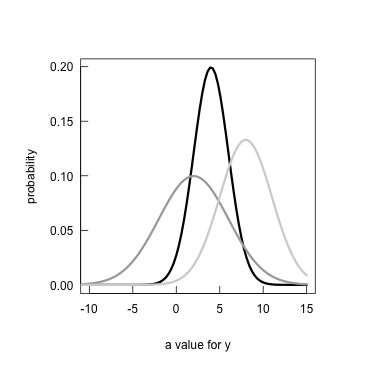
\includegraphics[width=\textwidth]{lectures/day_9_refreshing_glm/figures/unnamed-chunk-2-1.png}
            \end{figure}
        \end{column}
    \end{columns}
    \vspace{0.3cm}
    
    \[
    N(x) = P(Y = y; \mu, \sigma^2) = \frac{1}{\sqrt{2 \pi \sigma^2}} e^{\frac{-(y - \mu)^2}{2 \sigma^2}}
    \]
\end{frame}

\begin{frame}[fragile]
    \frametitle{Normal Distribution}
    \large
    \begin{columns}
        \begin{column}{0.5\textwidth}
            The normal distribution describes Gaussian processes where many independent processes add up to produce an effect
        \end{column}
        \begin{column}{0.5\textwidth}
            \begin{figure}
            \centering
            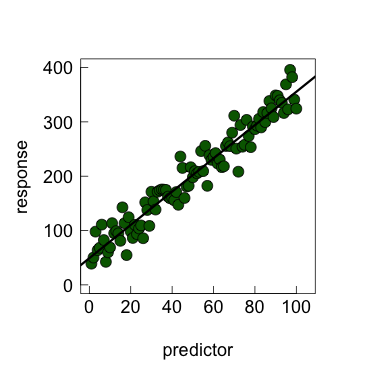
\includegraphics[width=\textwidth]{lectures/day_9_refreshing_glm/figures/unnamed-chunk-3-1.png}
            \end{figure}
        \end{column}
    \end{columns}
    \vspace{0.3cm}
    
    \[
    N(x) = P(X = y_i; \mu = \beta_0 + \beta_1 \cdot x_i, \sigma^2) = \frac{1}{\sigma \sqrt{2 \pi}} e^{\frac{-(x - (\mu = \beta_0 + \beta_1 \cdot x_i))^2}{2 \sigma^2}}
    \]
\end{frame}

\begin{frame}[fragile]
\frametitle{Other continuous distributions}
    \begin{columns}
        \begin{column}{0.45\textwidth}
            \small
            \begin{figure}
                \centering
            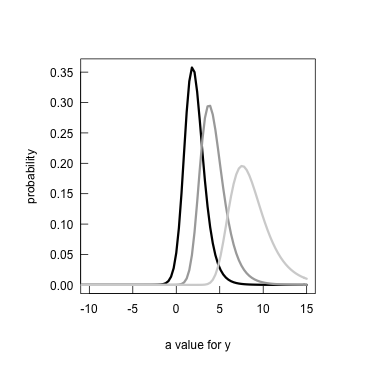
\includegraphics[width=0.8\textwidth]{lectures/day_9_refreshing_glm/figures/unnamed-chunk-4-1.png}
            \caption{T-Distribution}
            \end{figure}
            \small
            The t-distribution is used for estimating population parameters when the sample size is small or the population variance is unknown.
        \end{column}
        \begin{column}{0.45\textwidth}
            \begin{figure}
                \centering
                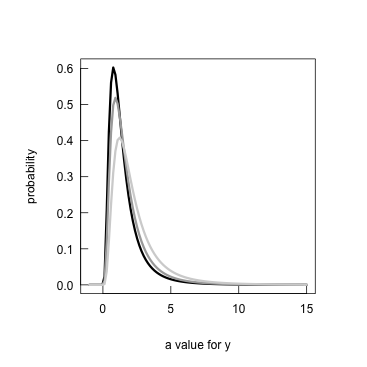
\includegraphics[width=0.8\textwidth]{lectures/day_9_refreshing_glm/figures/unnamed-chunk-5-1.png}
            \caption{F-Distribution}
            \end{figure}
            \small
            The F-distribution is used in the analysis of variance (ANOVA) for comparing variances and as null distribution for model testing.
        \end{column}
    \end{columns}
    
\end{frame}

\begin{frame}
    \frametitle{Distributions}
    \large
    Data with different characteristics produced by other processes exist:\\
    These have their own distributions
    \normalsize
    \begin{table}
        \begin{tabular}{|llll|}
        \hline
        Normal & Bernoulli & Binomial & Poisson \\ 
        \hline
        Cauchy & Chi$^2$ & Exponential & Gamma \\
        Geometric & Hypergeometric & Logistic & Log-Normal \\
        Negative Binomial& Student-t & Uniform & Weibull \\
        \hline
\end{tabular}
\end{table}
    \vspace{0.2cm}
    \large
    ... and hundreds more
\end{frame}


\section{Binomial and Bernoulli Distributions}

\begin{frame}[fragile]
    \frametitle{Binomial Distribution}
    \large
    \begin{columns}
        \begin{column}{0.5\textwidth}
            Discrete distribution for $k$ successes in a series of $n$ trials, that can result in values between 0 and 1, with $mean = np$ and $variance = np(1 - p)$:
        \end{column}
        \begin{column}{0.5\textwidth}
            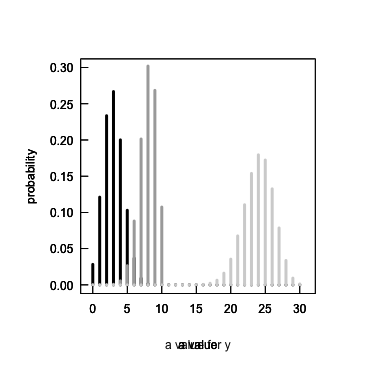
\includegraphics[width=\textwidth]{lectures/day_9_refreshing_glm/figures/unnamed-chunk-6-1.png}
        \end{column}
    \end{columns}
    \vspace{0.2cm}
    
    \[
    Binom(y) = P(Y = k; n, p) = \binom{n}{k} p^k(1 - p)^{n-k}
    \]

\end{frame}

\begin{frame}
\frametitle{Binomial Distribution}
    \large
    How often did something $k$ did happen or not $n-k = proportions$

    \[
    Binom(y) = P(Y = k; n, p = logit(\beta_0 + \beta_1 \cdot x))
    \]
    \[
    \left( n, p = \frac{e^{\beta_0 + \beta_1 \cdot x}}{1 + e^{\beta_0 + \beta_1 \cdot x}} \right) \left( \frac{e^{\beta_0 + \beta_1 \cdot x}}{1 + e^{\beta_0 + \beta_1 \cdot x}} \right)^k \left( 1 - \frac{e^{\beta_0 + \beta_1 \cdot x}}{1 + e^{\beta_0 + \beta_1 \cdot x}} \right)^{n-k}
    \]
    \vspace{0.2cm}
    
    \textit{e.g. Number of survivors from a fixed initial number of male offspring at high vs. low temperature}
\end{frame}

\begin{frame}[fragile]
    \frametitle{Bernoulli Distribution}
    \large
    \begin{columns}
        \begin{column}{0.5\textwidth}
            A special case of the binomial distribution where $n = 1$. The outcome can only be 0 or 1, is discrete and has a mean $p$ and a variance $p(1-p)$. \textbf{Not Independent}.
        \end{column}
        \begin{column}{0.5\textwidth}
            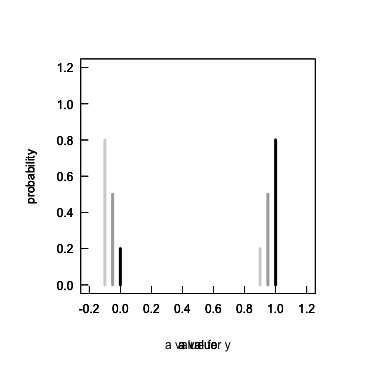
\includegraphics[width=\textwidth]{lectures/day_9_refreshing_glm/figures/unnamed-chunk-7-1.png}
        \end{column}
    \end{columns}
    
    
    \[
    Bern(y) = P(Y = k; p) = p^k(1-p)^{1-k}, \quad k \in \{0,1\}
    \]
    \[
    \begin{cases}
        p & \text{if} k = 1\\
        1 - p & \text{if} k = 0
    \end{cases}
    \]
\end{frame}

\begin{frame}
    \frametitle{Bernoulli Distribution}
    \large
    \begin{columns}
        \begin{column}{0.5\textwidth}
            Desribes experiments with a binary outcome:\\
            yes or no, 1 or 0, presence or absence, female or male
        \end{column}
        \begin{column}{0.5\textwidth}
            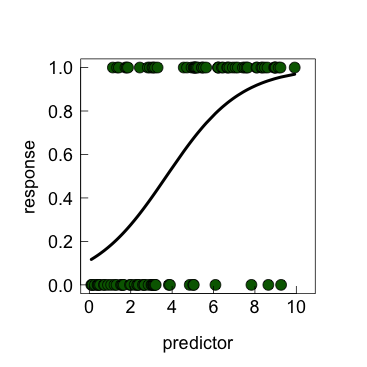
\includegraphics[width=\textwidth]{lectures/day_9_refreshing_glm/figures/unnamed-chunk-8-1.png}
        \end{column}
    \end{columns}
\[
\text{Bern}(y) = P(Y = k \;;\; p = \text{logit}(\beta_0 + \beta_1 \cdot x)) =
\]
\[
\begin{cases} 
\frac{e^{\beta_0 + \beta_1 \cdot x}}{1 + e^{\beta_0 + \beta_1 \cdot x}} & \text{if } k = 1, \\
1 - \frac{e^{\beta_0 + \beta_1 \cdot x}}{1 + e^{\beta_0 + \beta_1 \cdot x}} & \text{if } k = 0.
\end{cases}
\]

\end{frame}
\begin{frame}[fragile]
    \frametitle{Difference between Bernoulli and Binomial}
    \large
    \begin{columns}
        \begin{column}{0.5\textwidth}
            \textbf{Bernoulli:}\\
            Only one trial (Yes/No outcome).
            \vspace{0.2cm}
            
            \textit{What is the probability of k = 1 or k = 0 in a single trial we pursue?}
        \end{column}
        \begin{column}{0.5\textwidth}
            \textbf{Binomial:}\\
            More than 1 trial (multiple yes or no).
            \vspace{0.2cm}
            
            \textit{What is the probability of k successes when we pursue a tiral n times?}
        \end{column}
    \end{columns}
\end{frame}

\section{Poisson Distribution}

\begin{frame}[fragile]
    \frametitle{Poisson Distribution}
    \large
    \begin{columns}
        \begin{column}{0.5\textwidth}
            A distribution for discrete values between 0 and \textit{inf}, with mean = variance = \lambda
        \end{column}
        \begin{column}{0.5\textwidth}
            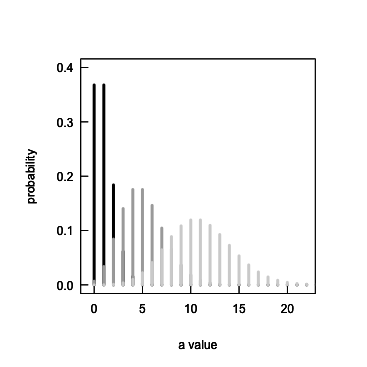
\includegraphics[width=\textwidth]{lectures/day_9_refreshing_glm/figures/unnamed-chunk-9-1.png}
        \end{column}
    \end{columns}

    \[
    Pois(y) = P(Y = k; \lambda) = \frac{\lambda^k e^{-\lambda}}{k!}
    \]
\end{frame}

\begin{frame}
    \frametitle{Poisson Distribution}
    \large
    \begin{columns}
        \begin{column}{0.5\textwidth}
            As the binomial, a count distribution:\\
            How often did something k happen in a given time?
            \vspace{0.2cm}

            \textit{e.g. Eggs laid per day, Animals counted per time or area}
        \end{column}
        \begin{column}{0.5\textwidth}
            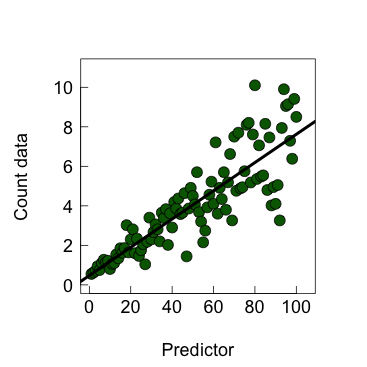
\includegraphics[width=\textwidth]{lectures/day_9_refreshing_glm/figures/unnamed-chunk-10-1.png}
        \end{column}
    \end{columns}

    \[
    Pois(y) = P(Y = k; \lambda = log(\beta_0 + \beta_1 \cdot x)) =
    \]
    \[
    \frac{log(\beta_0 + \beta_1 \cdot x)^k e^{-log(\beta_0 + \beta_1 \cdot x)}}{k!}
    \]
\end{frame}

\begin{frame}
    \frametitle{Mean - Variance Relationships}
    \begin{columns}
        \begin{column}{0.7\textwidth}
            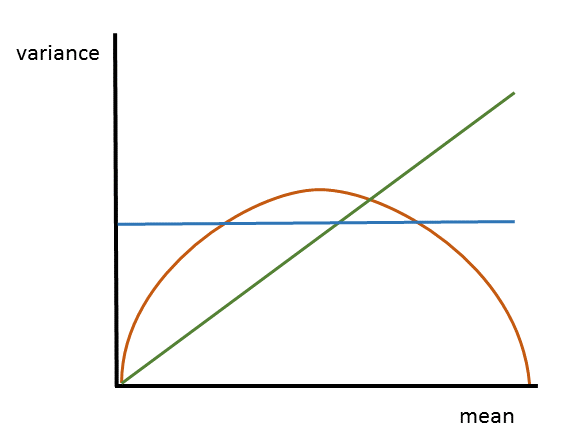
\includegraphics[width=\textwidth]{lectures/day_9_refreshing_glm/figures/mean-variance.png}
        \end{column}
        \begin{column}{0.3\textwidth}
            \textbf{Binomial (red)} \\
            \textbf{Poisson (green)} \\
            \textbf{Normal (blue)} \\
        \end{column}
    \end{columns}
    
\end{frame}

\section{GLM Structure}

\begin{frame}[fragile]
    \frametitle{Generalized Linear Model (GLM)}
    \textbf{A GLM is specified by three components:}\\
    1) An assumption about the distribution of the response variable and its parameters:
    \[
    Y \sim N(\mu, \sigma^2)
    \]
    \[
    E(Y) = \mu \text{ and } var(Y) = \sigma
    \]
    2) Specification of the linear predictor:
    \[
    \mu = \eta(X_1, ... , X_n) = \beta X
    \]
    3) Specification of the link function:
    \[
    link(\mu)
    \]
\end{frame}

\begin{frame}[fragile]
    \frametitle{Link Function}
    \large
    \begin{columns}
        \begin{column}{0.5\textwidth}
            Apparently, we build a regression model by attaching the linear model to some distribution parameters.\\
            \textit{The link function connects the linear predictor to the distribution parameters, ensuring that the predicted values follow the assumed distribution.}
        \end{column}
        \begin{column}{0.5\textwidth}
        From Dormann (2017):
            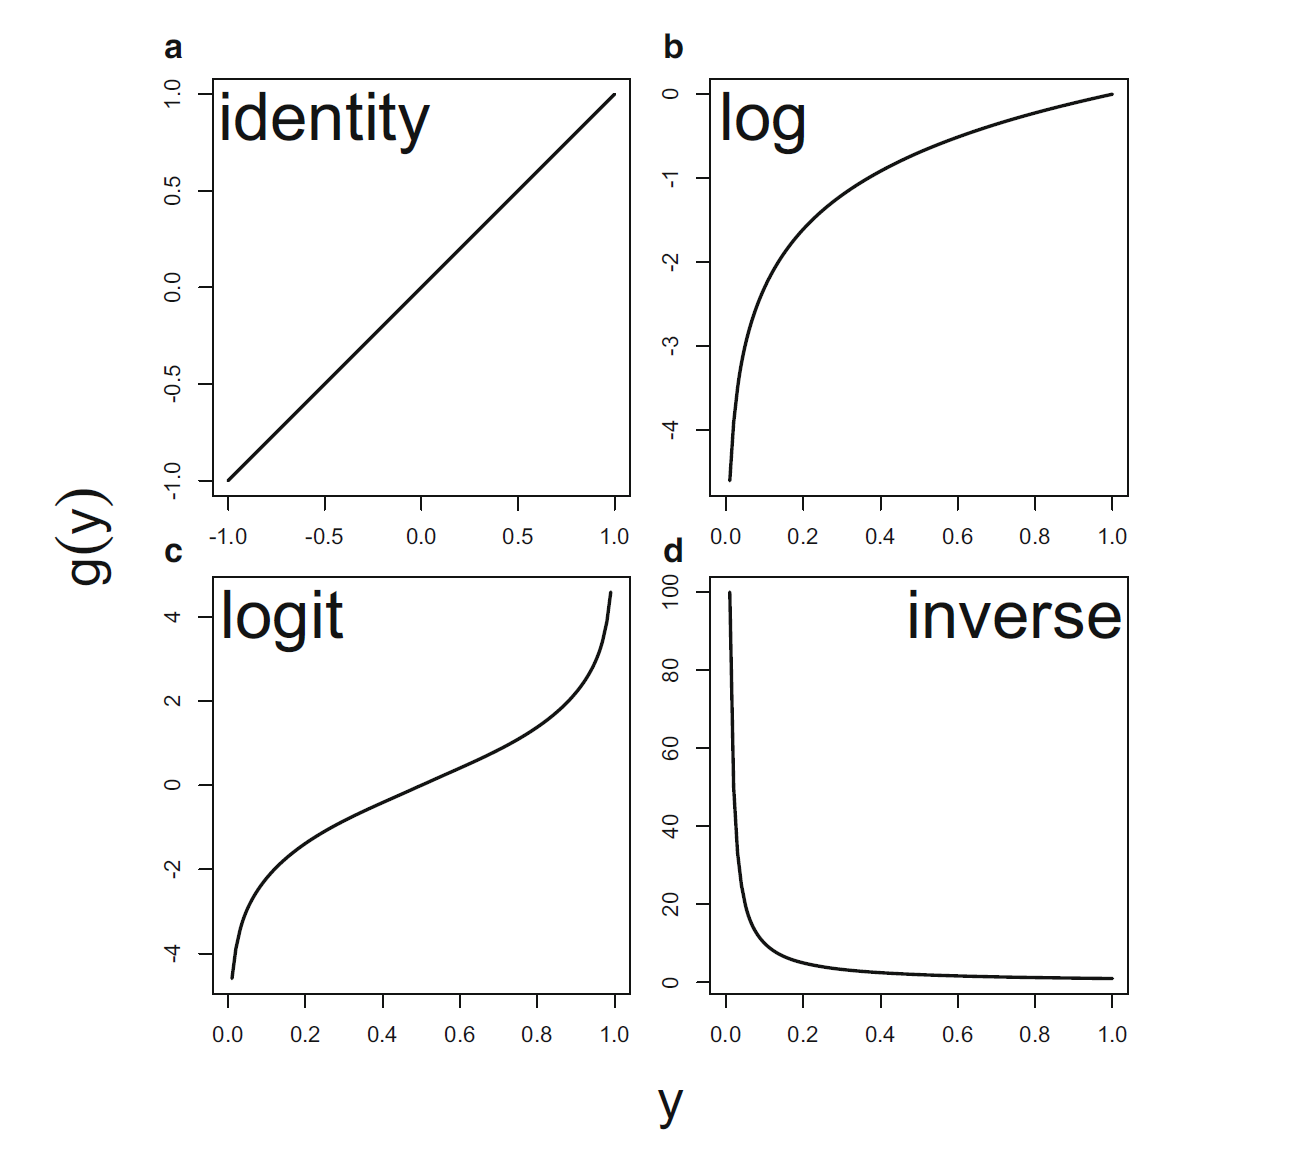
\includegraphics[width=\textwidth]{lectures/day_9_refreshing_glm/figures/links.png}
        \end{column}
    \end{columns}
\end{frame}

\begin{frame}[fragile]
    \frametitle{A Binomial Model for Proportion Data}
    \begin{columns}
        \begin{column}{0.5\textwidth}
        \scriptsize
            \begin{VerbatimIN}[numbers=left,numbersep=6pt]
daphnia$prop <-
daphnia$lebend/daphnia$total
            \end{VerbatimIN}
        \large
        Values between 0 and 1\\
        largest variance in the middle
        \end{column}
        \begin{column}{0.5\textwidth}
            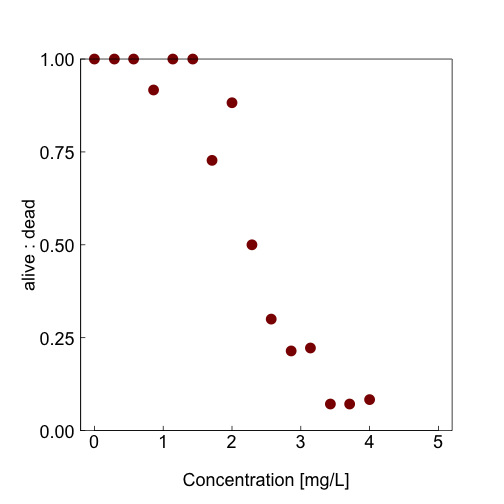
\includegraphics[width=\textwidth]{lectures/day_9_refreshing_glm/figures/unnamed-chunk-13-1.png}
        \end{column}
    \end{columns}
\end{frame}

\begin{frame}[fragile]
    \frametitle{A wrong linear regression model}
    \begin{columns}
        \begin{column}{0.5\textwidth}
        \scriptsize
            \begin{VerbatimIN}[numbers=left,numbersep=6pt]
normal <-
lm(prop ~ S, data=daphnia)
            \end{VerbatimIN}
        \normalsize
        Predictions for a proportion are $>1$ and $<0$.\\
        The confidence interval is wrong too.
        \end{column}
        \begin{column}{0.5\textwidth}
            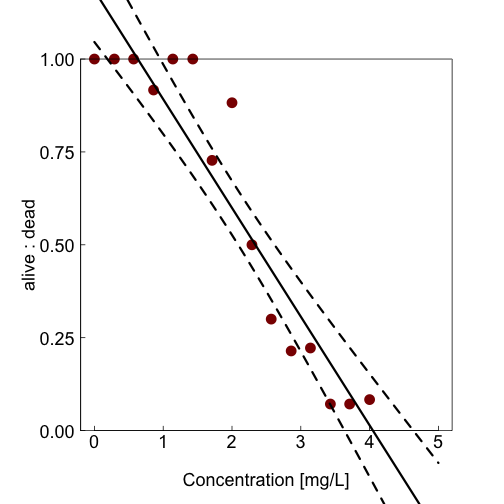
\includegraphics[width=\textwidth]{lectures/day_9_refreshing_glm/figures/unnamed-chunk-15-1.png}
        \end{column}
    \end{columns}
\end{frame}

\begin{frame}[fragile]
    \frametitle{The correct generalized linear model}
    \tiny
    \begin{VerbatimIN}[numbers=left,numbersep=6pt]
m.binomial <- glm(cbind(lebend, total - lebend) ~ S,  
                family = binomial(link = "logit"), 
                data = daphnia)
#successes = alive and failures = dead = total - alive
summary(m.binomial)
    \end{VerbatimIN}
    \begin{VerbatimOUT}[numbers=left,numbersep=6pt]
Call:
glm(formula = cbind(lebend, total - lebend) ~ S, family = binomial(link = "logit"), 
    data = daphnia)

Deviance Residuals: 
    Min       1Q   Median       3Q      Max  
-1.0611  -0.6261   0.2903   0.8255   1.4012  

Coefficients:
            Estimate Std. Error z value Pr(>|z|)    
(Intercept)   5.7031     0.8062   7.074 1.51e-12 ***
S            -2.3135     0.3132  -7.387 1.50e-13 ***
---
Signif. codes:  0 '***' 0.001 '**' 0.01 '*' 0.05 '.' 0.1 ' ' 1

(Dispersion parameter for binomial family taken to be 1)

    Null deviance: 157.141  on 14  degrees of freedom
Residual deviance:  10.734  on 13  degrees of freedom
AIC: 38.803

Number of Fisher Scoring iterations: 5
    \end{VerbatimOUT}
\end{frame}

\section{Binomial GLM Example}

\begin{frame}[fragile]
    \frametitle{}
    \Large
    \textbf{The logit-link function for binomial estimates:}
    \[
    logit(p) = \log\left(\frac{p}{1 - p}\right) = \beta_0 + \beta_1 \cdot x
    \]
\end{frame}

\begin{frame}
    \frametitle{The logit-link Function}
    \begin{columns}
        \begin{column}{0.5\textwidth}
            The logit-link allows to fit the non-linear relationship between X and y as a linear relationship $a + b \cdot x$ on the logit-scale.
            \vspace{0.2cm}
            
            On the logit-scale, values $>1$ and $<0$ are possible.
            \begin{align*}
                &logit(0) = log(0/(1-0)) = -Inf \\
                &logit(0.5) = log(0.5/(1-0.5)) = 0 \\
                &logit(1) = log(1/(1-1)) = +Inf
            \end{align*}
            No negative values in the log function allowed: Restrictions on the data
        \end{column}
        \begin{column}{0.5\textwidth}
            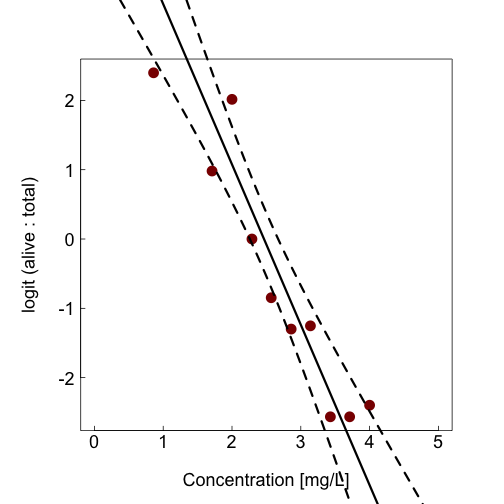
\includegraphics[width=\textwidth]{lectures/day_9_refreshing_glm/figures/unnamed-chunk-17-1.png}
        \end{column}
    \end{columns}
\end{frame}

\begin{frame}[fragile]
    \frametitle{Inverse Link / Response Function}
    \large
    The logit-values are \textbf{NOT} the y-values, but the fitted proportion values on the link-scale.\\
    \textit{We have to use the  inverses function to get back to the measurement scale.}
    \[
    logit^{-1}(p) = \frac{e^{\hat{\beta_0} + \hat{\beta_1} \cdot x}}{1 + e^{\hat{\beta_0} + \hat{\beta_1} \cdot x}}
    \]
\end{frame}

\begin{frame}
    \begin{center}
    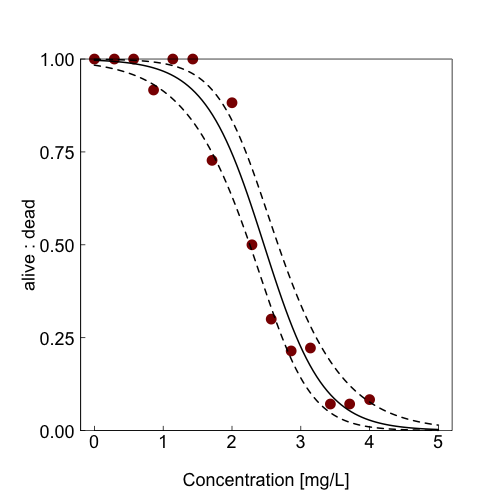
\includegraphics[width=0.65\textwidth]{lectures/day_9_refreshing_glm/figures/unnamed-chunk-18-1.png}
    \end{center}
    \begin{itemize}
    \centering
        \item Predictions in range
        \item Errors in range
    \end{itemize}
\end{frame}

\begin{frame}
    \frametitle{A Poisson Model for Count Data}
    \large
    \begin{columns}
        \begin{column}{0.5\textwidth}
            \textbf{Properties:}\\
            1) Discrete values, which are never $< 0$\\
            2) Higher variance for larger values
        \end{column}
        \begin{column}{0.5\textwidth}
            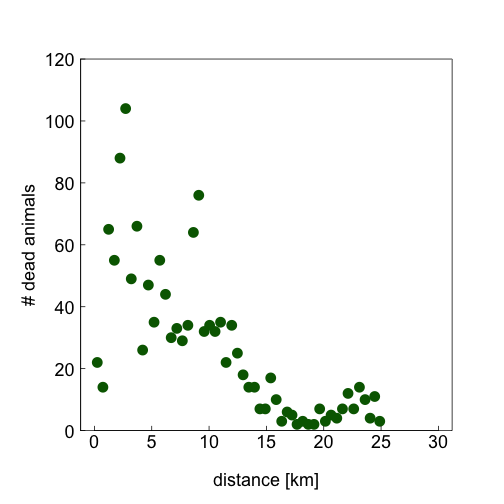
\includegraphics[width=\textwidth]{lectures/day_9_refreshing_glm/figures/unnamed-chunk-19-1.png}
        \end{column}
    \end{columns}
\end{frame}

\begin{frame}[fragile]
    \frametitle{A wrong Linear Regression Model}
    \begin{columns}
        \begin{column}{0.5\textwidth}
        \scriptsize
            \begin{VerbatimIN}[numbers=left,numbersep=6pt]
normal <- 
lm(dead ~ Distance, 
data = roadkill
            \end{VerbatimIN}
        \large
        Negative predicted counts of dead animals.\\
        Also: Negative errors same variance everywhere.
        \end{column}
        \begin{column}{0.5\textwidth}
            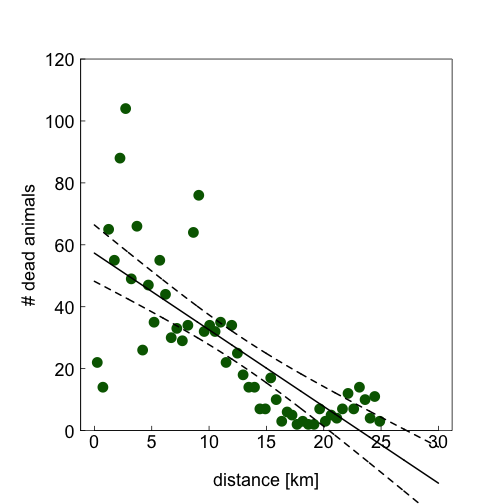
\includegraphics[width= \textwidth]{lectures/day_9_refreshing_glm/figures/unnamed-chunk-21-1.png}
        \end{column}
    \end{columns}
\end{frame}

\begin{frame}[fragile]
    \frametitle{The correct Generalized Linear Model}
    \tiny
    \begin{VerbatimIN}[numbers=left,numbersep=6pt]
m.poisson <- glm(Dead ~ Distance, 
                family = poisson(link = "log"),  
                data = roadkill)
summary(m.poisson)        
    \end{VerbatimIN}
    \begin{VerbatimOUT}[numbers=left,numbersep=6pt]
Call:
glm(formula = Dead ~ Distance, family = poisson(link = "log"), 
    data = roadkill)

Deviance Residuals: 
    Min       1Q   Median       3Q      Max  
-8.1100  -1.6950  -0.4708   1.4206   7.3337  

Coefficients:
             Estimate Std. Error z value Pr(>|z|)    
(Intercept)  4.316485   0.043220   99.87   <2e-16 ***
Distance    -0.105851   0.004387  -24.13   <2e-16 ***
---
Signif. codes:  0 '***' 0.001 '**' 0.01 '*' 0.05 '.' 0.1 ' ' 1

(Dispersion parameter for poisson family taken to be 1)

    Null deviance: 1071.4  on 51  degrees of freedom
Residual deviance:  390.9  on 50  degrees of freedom
AIC: 634.29

Number of Fisher Scoring iterations: 4        
    \end{VerbatimOUT}
\end{frame}

\begin{frame}[fragile]
    \frametitle{}
    \Large
    \textbf{The log-link function for poisson estimates:}
    \[
    \textit{log}(\lambda) = \ln(\lambda) = \beta_0 + \beta_1 \cdot x
    \]
\end{frame}

\begin{frame}
    \frametitle{The log-link function}
    \begin{columns}
        \begin{column}{0.5\textwidth}
            The log-link changes the non-linear relationship between the data (now on the log-scale) to a linear relationship: $a + b \cdot x$.
            \vspace{0.2cm}
            
            Again values $< 0$ are possible on the log-scale.
            \begin{align*}
&log(0) = -Inf\\
&log(1) = 0 \\
&log(10) = 2.3
            \end{align*}
        \end{column}
        \begin{column}{0.5\textwidth}
            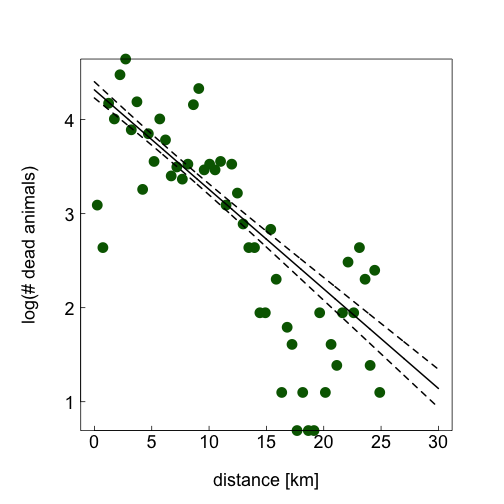
\includegraphics[width=\textwidth]{lectures/day_9_refreshing_glm/figures/unnamed-chunk-23-1.png}
        \end{column}
    \end{columns}
\end{frame}


\begin{frame}
    \frametitle{}
    \begin{center}
    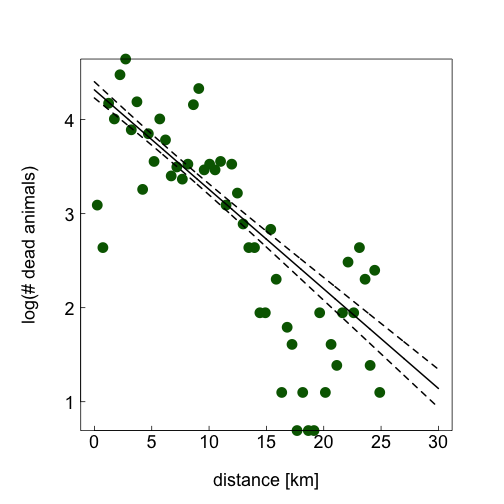
\includegraphics[width=0.65\textwidth]{lectures/day_9_refreshing_glm/figures/unnamed-chunk-24-1.png}
    \vspace{0.3cm}
    
    \large
    log(-5) is not allowed but such values are not measured 
    \end{center}
\end{frame}

\begin{frame}
    \frametitle{Inverse link function}
    \large
    The log-values are \textbf{NOT} the y-values, but the expected values from a Poisson distribution with a certain $\lambda$ on the log-scale.\\
    \textit{Use the inverse function to get back to the measurement scale}

    \[
    log^{-1}(\lambda) = e^{\hat{\beta_0} + \hat{\beta_1} \cdot x}
    \]
\end{frame}

\begin{frame}
    \frametitle{}
    \begin{center}
        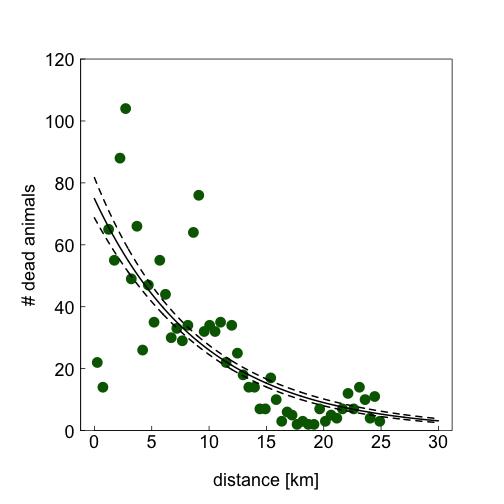
\includegraphics[width=0.65\textwidth]{lectures/day_9_refreshing_glm/figures/unnamed-chunk-25-1.png}
    \end{center}
    \begin{itemize}
    \centering
        \item Predictions in range
        \item Errors in range
    \end{itemize}
\end{frame}
\section{Diagnostics for GLMs}

\begin{frame}[fragile]
    \frametitle{Diagnostics for GLMs}
    \large
    \textbf{Diagnostics:}
    \begin{itemize}
        \item The \textbf{fab four} (residual plots, etc.) don't apply directly, as resiudals are by definition not normally distributed
        \item Studentized residuals at the link scale
        \item Simulation approaches (e.g. using DHARMa)
    \end{itemize}
\end{frame}

\begin{frame}[fragile]
    \large \textbf{There is a strong pattern in the residuals:}
    \scriptsize
    \begin{VerbatimIN}[numbers=left,numbersep=6pt]
stud.res <- rstudent(m.poisson)
fitted <- predict(m.poisson, type="link")
plot(stud.res ~ fitted, pch = 16, las = 1, cex.lab = 1.5, 
     ylab = "Studentized Residuals", xlab = "fitted values")
abline(h = 0, col = "grey")
    \end{VerbatimIN}
    \begin{center}
        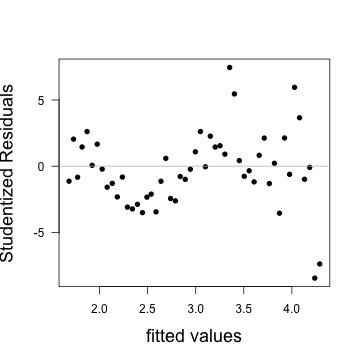
\includegraphics[width=0.5\textwidth]{lectures/day_9_refreshing_glm/figures/unnamed-chunk-26-1.png}
    \end{center}
\end{frame}

\begin{frame}
    \frametitle{}
    \Large
    \begin{center}
        \textbf{There are two additional checks required:}
    \begin{itemize}
        \item Check for dispersion
        \item Check for zero-inflation
    \end{itemize}
    \end{center}   
\end{frame}

\begin{frame}
    \frametitle{Check for Dispersion:}
    \begin{columns}
        \begin{column}{0.5\textwidth}
            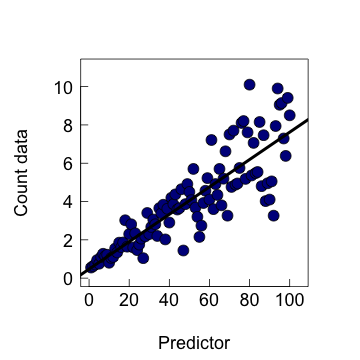
\includegraphics[width=\textwidth]{lectures/day_9_refreshing_glm/figures/unnamed-chunk-27-1.png}
        \end{column}
        \begin{column}{0.5\textwidth}
           \textbf{Mean and Variance are related to each other:}\\
            If the distribution-specific relationship is not the assumed one for the data, over- or under-dispersion occurs (too fast or slow change in variance with the mean)
        \end{column}
    \end{columns}
\end{frame}

\begin{frame}[fragile]
    \frametitle{Checking Dispersion in R}
    \begin{columns}
        \begin{column}{0.5\textwidth}
        \tiny
            \begin{VerbatimIN}[numbers=left,numbersep=6pt]
summary(m.poisson)$dispersion
            \end{VerbatimIN}
            \begin{VerbatimOUT}[numbers=left,numbersep=6pt]
[1] 1
            \end{VerbatimOUT}
            \begin{VerbatimIN}[numbers=left,numbersep=6pt]
m.poisson$deviance / m.poisson$df.residual
            \end{VerbatimIN}
            \begin{VerbatimOUT}[numbers=left,numbersep=6pt]
[1] 7.817937
            \end{VerbatimOUT}
            \normalsize
            This is the residual deviance by residual degrees of freedom. The value should be around 1.
        \end{column}
        \begin{column}{0.5\textwidth}
            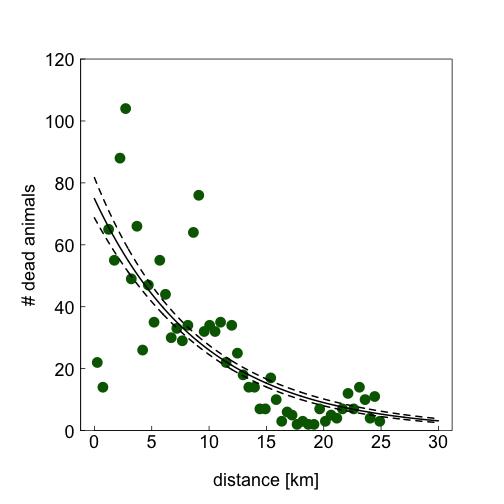
\includegraphics[width=\textwidth]{lectures/day_9_refreshing_glm/figures/unnamed-chunk-29-1.png}
        \end{column}
    \end{columns}
    \vspace{0.2cm}
    
    \textbf{Here, too much variance occurs at higher predicted values.}
\end{frame}

\begin{frame}
    \frametitle{Check for Zero-Inflation}
    \large
    \textbf{Observed zeros may deviate from the assumed distribution:}\\
    If there are too many (zero-inflation) or too few (zero-truncation) compared to the model assumption, it indicates a mismatch that can affect model performance
\end{frame}

\begin{frame}[fragile]
    \large
    \frametitle{Residual Checks in R: DHARMa}
    \textbf{Residual Checks using Simulations:}
    \begin{itemize}
        \item[Step 1:] Simulate responses under the postulated model you want to test
        \item[Step 2:] Repeat this multiple (many, many...) times 
        \item[Step 3:] Create a distribution of the simulated residuals
        \item[Step 4:] Compare the new against the observed residuals to check for irregularities  
    \end{itemize}
    \vspace{0.2cm}
    
    \textit{If the model is correctly specified, the simulated and observed values should be similar}
\end{frame}

\begin{frame}[fragile]
    \frametitle{Residual Checks in R: DHARMa}#
    \scriptsize
    \begin{VerbatimIN}[numbers=left,numbersep=6pt]
library(DHARMa)
sim <- simulateResiduals(m.poisson, n = 250)
plot(sim)
    \end{VerbatimIN}
    \begin{center}
        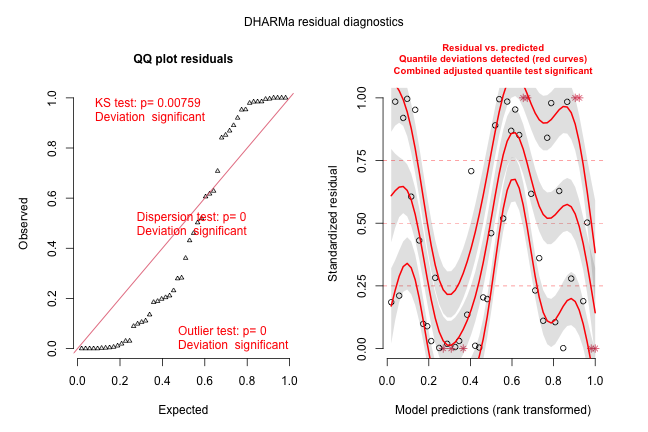
\includegraphics[width=0.8\textwidth]{lectures/day_9_refreshing_glm/figures/unnamed-chunk-30-1.png}
    \end{center}
\end{frame}

\begin{frame}[fragile]
    \frametitle{Residual Checks in R: Dispersion}
    \scriptsize
    \begin{columns}
        \begin{column}{0.4\textwidth}
            \begin{VerbatimIN}[numbers=left,numbersep=6pt]
testDispersion(sim)
            \end{VerbatimIN}
        \end{column}
        \begin{column}{0.6\textwidth}
            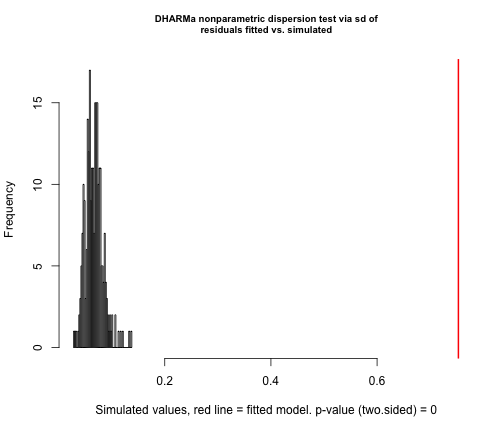
\includegraphics[width=\textwidth]{lectures/day_9_refreshing_glm/figures/unnamed-chunk-31-1.png}
        \end{column}
    \end{columns}

    \begin{VerbatimOUT}[numbers=left,numbersep=6pt]
    DHARMa nonparametric dispersion test via sd of residuals fitted 
    vs. simulated

data:  simulationOutput
dispersion = 11.214, p-value < 2.2e-16
alternative hypothesis: two.sided
    \end{VerbatimOUT}
\end{frame}

\begin{frame}[fragile]
    \frametitle{Residual Checks in R: Zero-inflation}
    \scriptsize
    \begin{columns}
        \begin{column}{0.4\textwidth}
            \begin{VerbatimIN}[numbers=left,numbersep=6pt]
testZeroInflation(sim)
            \end{VerbatimIN}
        \end{column}
        \begin{column}{0.6\textwidth}
            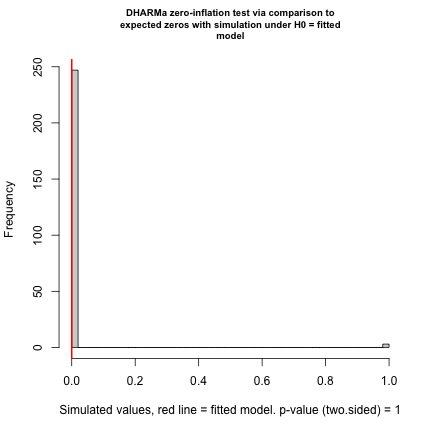
\includegraphics[width=0.9\textwidth]{lectures/day_9_refreshing_glm/figures/unnamed-chunk-32-1.png}
        \end{column}
    \end{columns}

    \begin{VerbatimOUT}[numbers=left,numbersep=6pt]
    DHARMa zero-inflation test via comparison to expected zeros with
    simulation under H0 = fitted model

data:  simulationOutput
ratioObsSim = 0, p-value = 1
alternative hypothesis: two.sided
    \end{VerbatimOUT}
\end{frame}

\begin{frame}
    \frametitle{General Advice}
    \large
    These extra checks are generally less important in GLM's that assume distributions with a dispersion or scale parameter (e.g. negative binomial distribution).
\end{frame}

\begin{frame}
    \frametitle{Spoiler Alert...}
    \centering
    \huge\textbf{glm + lmm = glmm}
    \vspace{0.2cm}
    
    \normalsize More on that next week.
\end{frame}
\begin{frame}[fragile]
    \frametitle{Recapitulation Week 9}
    Key concepts covered today:
    \begin{itemize}
        \item Poisson, Bernoulli, and Binomial distributions
        \item GLM structure: link functions, inverse function and linear predictors
        \item Mean-variance relationships
        \item Diagnosing GLMs: overdispersion and zero-inflation
    \end{itemize}
    Todays exercises:
    \begin{itemize}
        \item Work through GLM Demo
        \item Exercises on fitting GLMs
    \end{itemize}
\end{frame}

\end{document}
